\chapter{Molecular Dynamics and sampling techniques (Lecture Wed 15 April)}



\paragraph{Ergodic hypotesis} of equilibrium statistical mechanics, which establishes the equivalence between \textit{ensemble averages} and \textit{time averages} of macroscopic observables in the microcanonical ensemble.
i.e. \textit{given unlimited time, a trjectory a will sample the whole of phase space}.

\begin{align*}
    A_{time} &= \lim_{T\rightarrow + \infty}\, \int_{t=0}^{t= T} \,dt  \, A [\mathbf{r}(t), \mathbf{p}(t)] \\
    A_{ensemble} &= \int_{\Omega} d\mathbf{r}d\mathbf{p} \,\,A(\mathbf{r}, \mathbf{p})\, p(\mathbf{r}, \mathbf{p}) \\
A_{time} &\equiv A_{ensemble}\quad  \text{Ergodic Hypotesis}
\end{align*}

\begin{figure}[H]
    \centering
    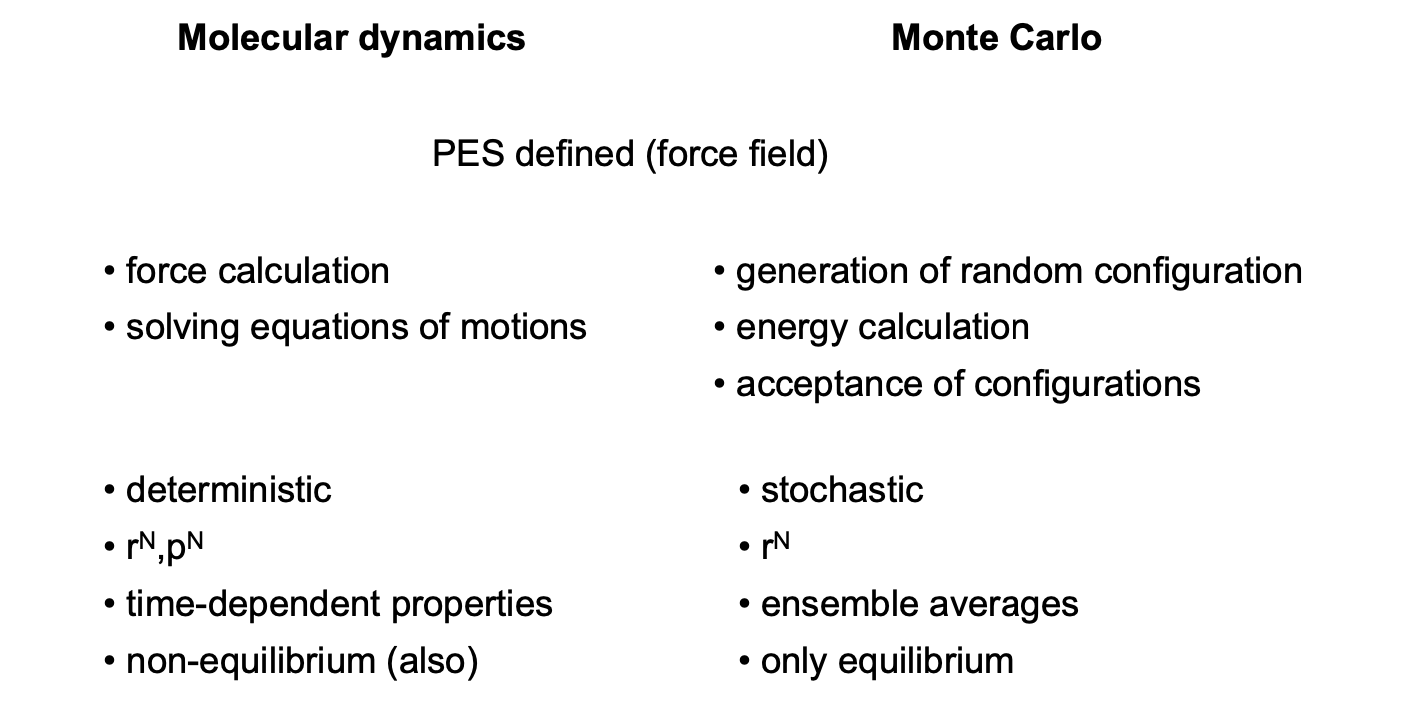
\includegraphics[width=\textwidth]{slides/simulations/dinamics_vs_montecarlo.png}
    \caption{Two ways to explore the PES: molecular dynamics (MD) vs Montecarlo sampling}
\end{figure}



\section{Pure Montecarlo sampling of the PES}
Metropolis sampling (Monte Carlo) is used as a method to generate configurations of molecular systems according to the Boltzmann distribution:
$$P(x) \propto e^{-\beta U(x)}$$
This is used to compute thermodynamic averages (energy, pressure, structure, etc.) without solving dynamics explicitly (as in MD).

Historically, Monte Carlo (especially Metropolis MC) was a central tool for studying liquid-phase systems, especially before modern large-scale MD.
It was essential for parameter development. I briefly mentioned about the van der Waals parameters, the Lennard-Jones potential, and we also mentioned some of the charge parameters.
I told you that we need to optimize it based on the simulations because of the lack of the polarization. You need to adjust some of the parameters. 

Then of course, you can go to more complex systems: polymers, or multiphases, membranes, and so on. These are some potential applications.
In the original Metropolis, you make a random move of a random particle, but obviously there are tricks to bias the simulation. For example, if you want to expand the membrane in a specific direction, you can implement some kind of factors that you include when you accept configurations and then you correct with them when you compute the averages.

\begin{figure}[H]
    \centering
    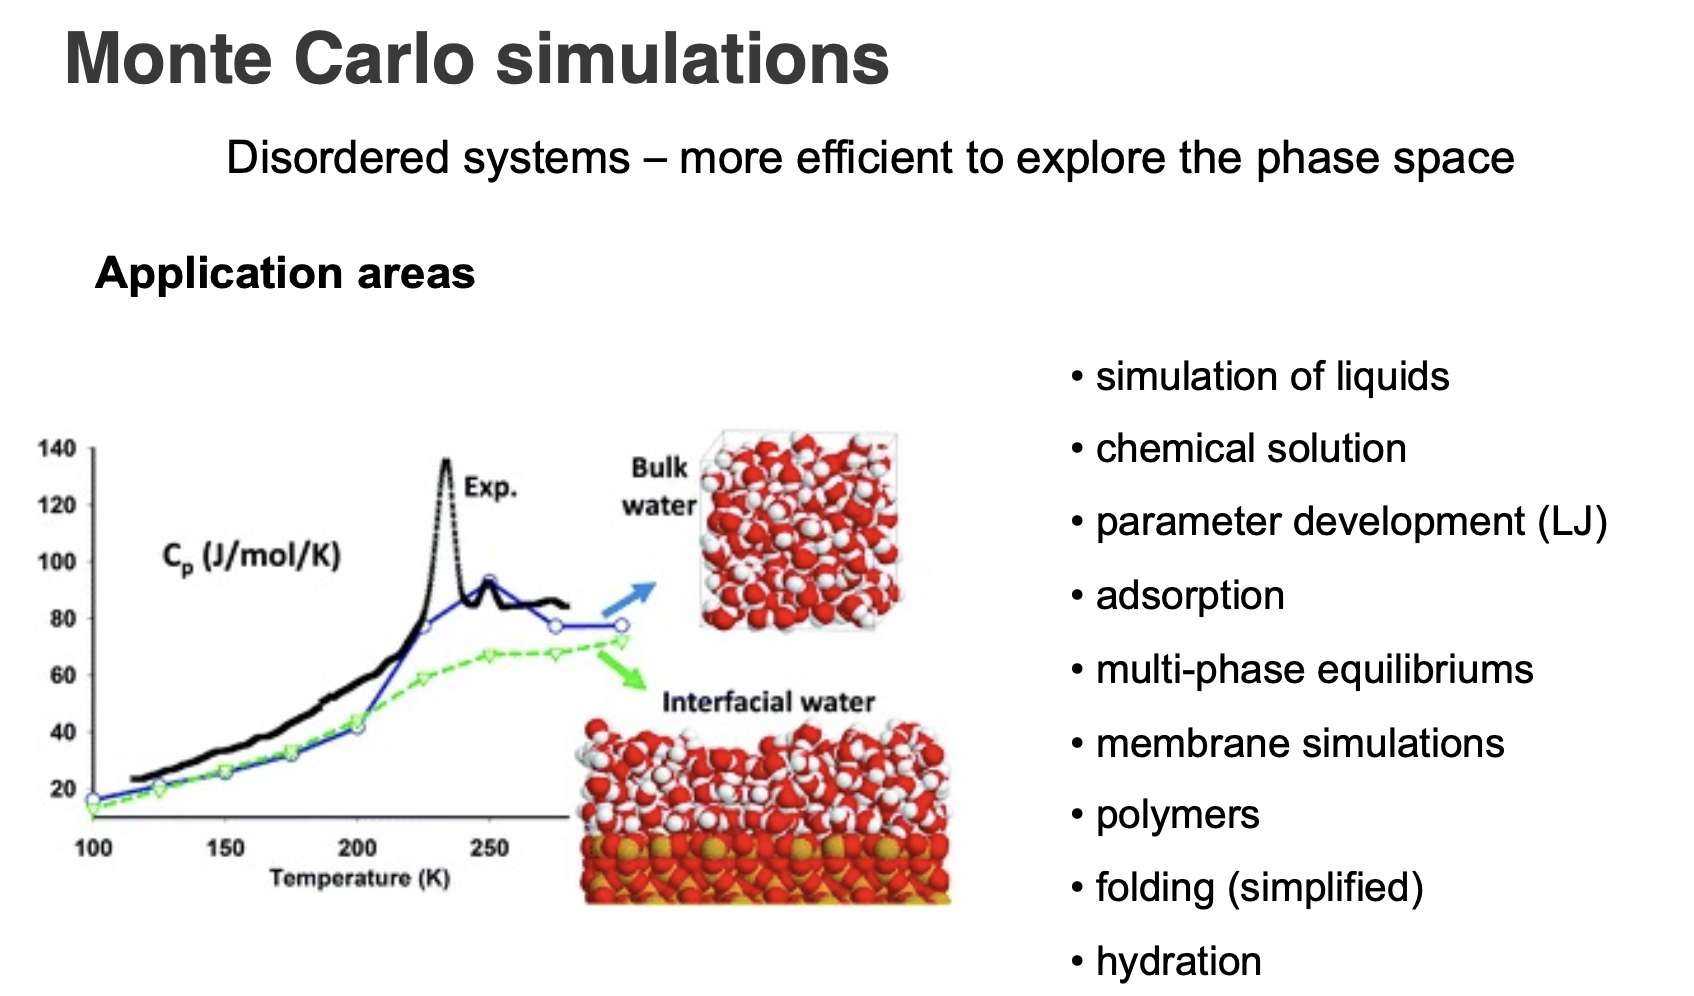
\includegraphics[width=0.6\textwidth]{slides/simulations/MC_applications.png}
\end{figure}

\section{Molecular Dynamics}
Application area is basically broader (w.r.t. Montecarlo-based sampling methods).
Obviously, you generate conformational ensembles,like with Monte Carlo. But additionally, you can get many \textit{dynamical aspects} of functionalities, for example, diffusion.
MD is widely used simply because computers got more powerful, so the integration itself can be done faster and so we can reach out to biologically meaningful temporal scales.


\begin{figure}[H]
    \centering
    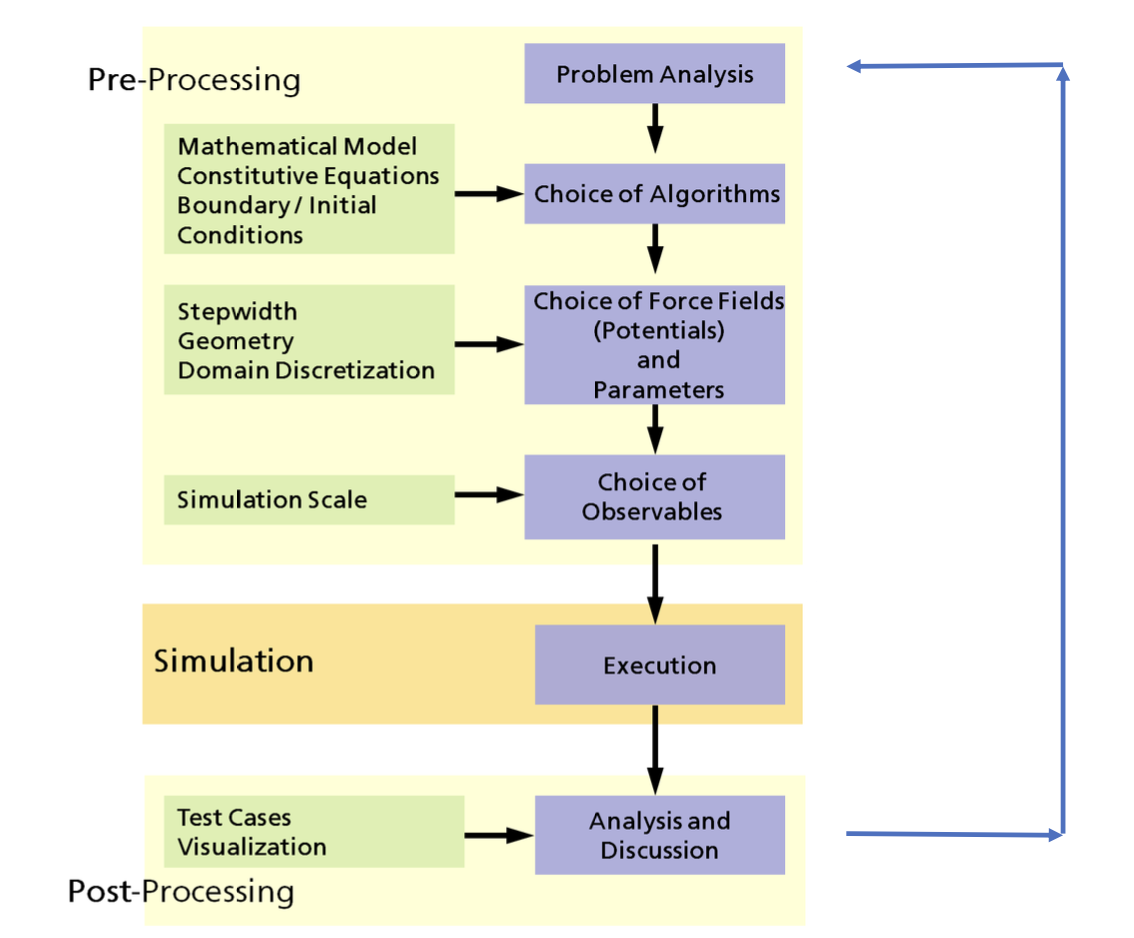
\includegraphics[width=\textwidth]{slides/simulations/MD_pipeline.png}
\end{figure}


\paragraph{How to choose the initial condition}
How do you choose the initial condition? Nowadays, you can ask AlphaFold to generate one for you. So you get it, you press the start button. Simple.
No. I mean, you can start, but what you will see immediately is that you put your AlphaFold structure into the simulation and it explodes. 
It is not AlphaFold problem, this happens also if you take your initial condition from X-ray crystallography from the PDB.
\textbf{The issue is that the experimental or predicted structure is a minimum of some effective landscape, but not necessarily a minimum of \textit{your} landscape.} Formally,

$$
\nabla U_{\text{experiment}}(x_0)=0 \quad \text{but} \quad \nabla U_{\text{FF}}(x_0)\neq 0
$$


\begin{figure}[H]
    \centering
    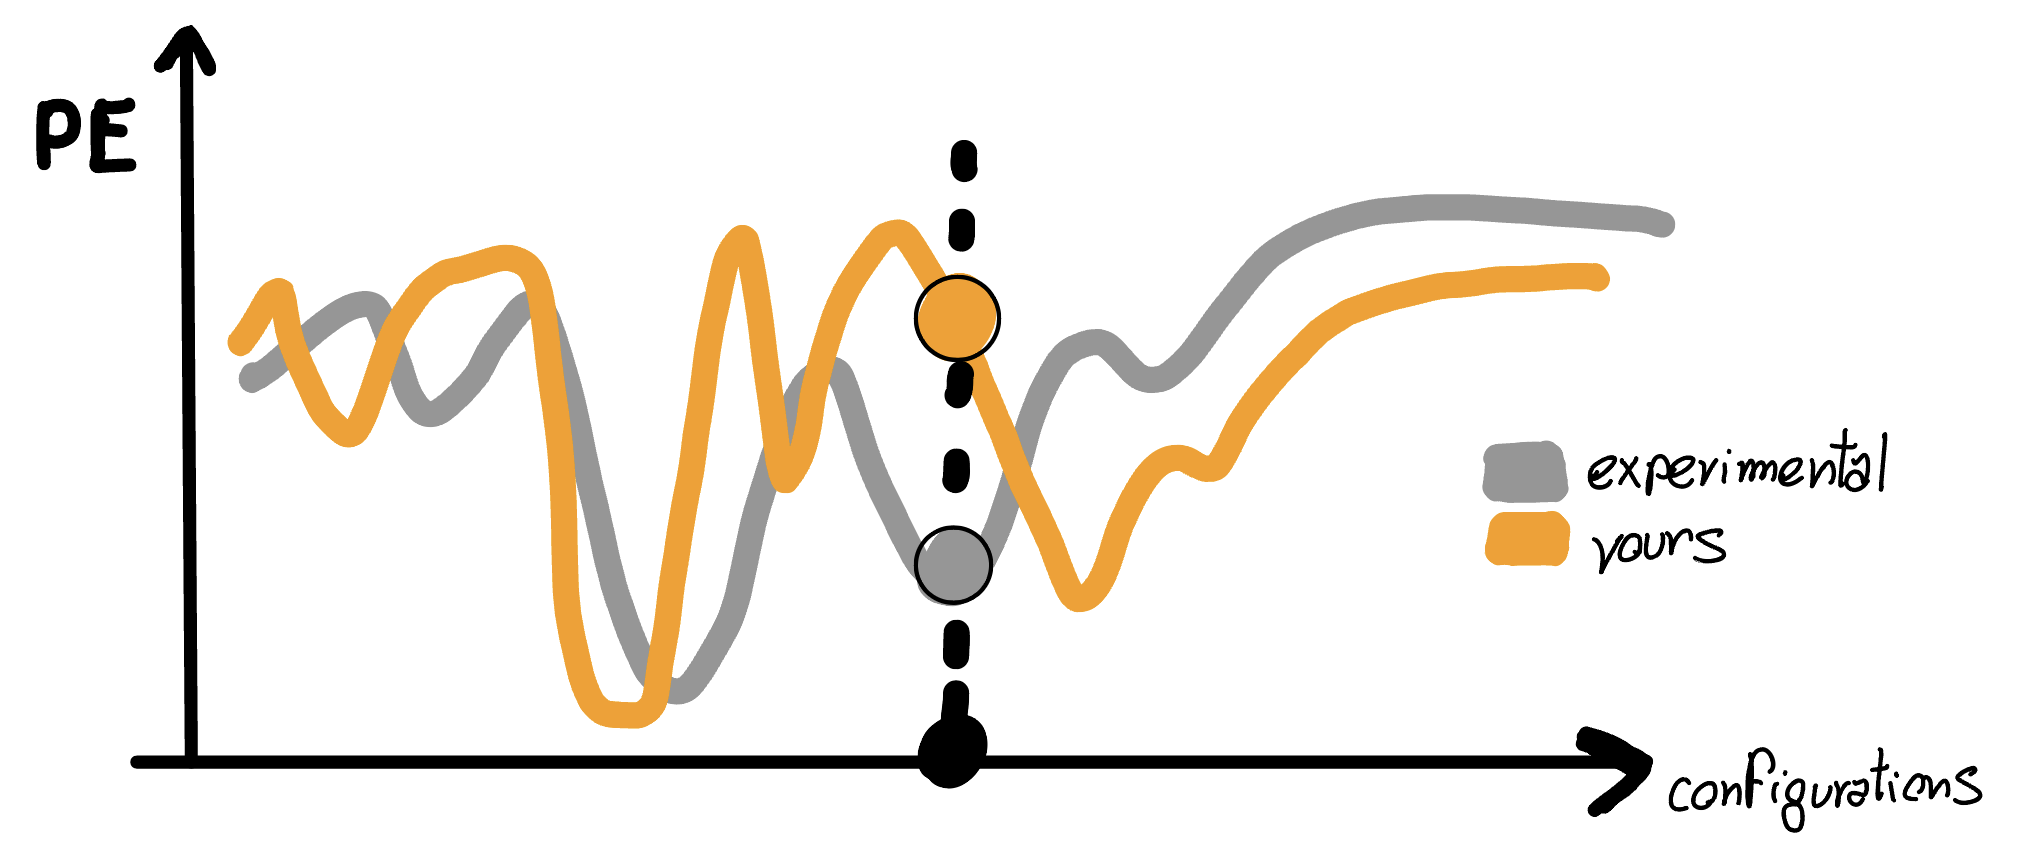
\includegraphics[width=0.7\textwidth]{slides/simulations/initial_condition.png}
\end{figure}

Maybe—maybe the initial, maybe AlphaFold, or maybe X-ray, or maybe NMR, whatever methodology—so they give you a minimum according to their method and this is here. But you start from the Amber force field. There is no guarantee that the two are compatible. That point could actually be very high on a slope in your force field.
When you plug that structure into your force field, the gradients of your force field could be steep, so the forces in the first few steps of the simulations are very strong and may cause the protein to explode.
Experimental structures are full of problems. First of all, there can be some atomic clashes, which produce very high Lennard-Jones repulsion wneh simulation starts. Also, there maybe some very unfavorable rotamers. 
You never start a simulation directly from raw structures. You must:

\begin{enumerate}
\item Preprocess (add hydrogens, fix missing atoms, assign protonation states)
\item \textbf{Energy minimization}: relax structure under the chosen force field, remove clashes
\item Equilibration: gradually heat system
\end{enumerate}

So you want to get this either to here or to here, to start from somewhere where your structure is reasonable, you don't expect anything funky in the first ten steps of the simulation. So therefore, to cut the long story short, what you do: you minimize it.

Your goal: get to a local minimum of your potential energy landscape in the proximity of where you started. For maximal efficiency you should adopt a multi-stage minimization strategy which incorporates several numerical methods:



So when you are far, very first you start with Steepest Descent and this is slow, but it's better to use because it will give you very small steps so you start coming towards here.

When you reach approximately—I mean these are not like, you know, stone-carved, but approximate values—so when you reach approximately like whatever one kilocalorie per mole per angstrom or below, then you try to switch to Conjugate Gradients, okay, that you—you fasten the process.

And then if you are lucky, you get around like 1/100 and then you change to Newton-Raphson and then you come to here. Of course you—you know, again, the rules are not rigid. But you will see that one can get so excited about the simulation—Oh, it's going, I see my I don't know arginine moving around—you know, you get passionate and you forget to look at your gradients.

This is a typical error of—not error but—but a typical thing that students normally do. So always when you start a voyage, you—you watch your maximum gradients. And also it's useful to—I mean the gradients are not uniformly distributed, there are some parts that are worse than others, maybe, you know, there are some clashes, the electron density map was not so whatever—I could tell long stories why it's so inhomogeneous, but the problems are inhomogeneous.

And—so it's worthwhile to look at Oh, my maximum gradient are absolutely I don't know 10,000 is on that hydrogen, what is going on? Quickly look at it in VMD or whatever you use, maybe you realize that you—you forgot to assign the hydrogen to something and that hydrogen is already in I don't know other part of the universe. So whatever, be careful, okay?



\paragraph{Solvating the system}
Then there are some other let's say recipes for being cautious, okay? And this is simply—we will speak about how to build the system, okay? Because until now we spoke about protein, but to make a good simulation, we need to build a system where the protein cannot be in vacuum, you need to put some solvents, maybe some ions, whatever.

This we will discuss how to do. But definitely when you optimize, when you generate your initial configuration for the simulation, you need to be very gradual in a sense that you first start with the solvents optimizing around the protein, then ions, then the flexible part, then the whole protein.

And until you reach that stage, you—you constrained the rest—don't move, because it may give you horrible results. Why? I just highlight one point. For example, when you—how you solvate your protein.

Obviously, you don't want to run a simulation prior to your protein simulation. You basically like in a—in a freezer part of the—the supermarket, you buy these little ice cubes. Whatever, ice cube of I don't know broccoli, ice cube of this. So this is how the water—solvents in general look like.

So people make simulations and they store it in large libraries. This comes together with your program. And basically you make a choice if you want the red or green or whatever. But this means that it's the configuration—pre-equilibrated configurations of that solvent, for example water, TIP3P, TIP4P, remember we discussed last week.

So you have a solution. But these are—this myriad of cubes, they are—they are made as pure, not for your protein. So basically, you know, you take your protein, then you—you buy the ice cubes, okay, you put I don't know hundred, whatever, okay?

Obviously you delete everything where you have protein atoms, you remain the rest. But what guarantee that this water that had ever seen in his life other waters, not this charged protein residues, that this would remain the same?

There is no—no guarantee. Furthermore, there is a guarantee that it should be different because the protein has an impact, has an electrostatic potential, whatever. So therefore, first the solvent, in order not to ruin your data, first the solvent has to adjust to whatever you have inside, the ions, because you'd better do a neutral system, and then only you let the protein to respond to everything.

So being cautious is like slow cooking, very—very slow thing to do, very cautiously thing to do. All logical, but very, you know, keep it.



\paragraph{Periodic Boundary Conditions}
So, okay. So in that manner, which may take a little while but all worth to minimize well your system. So then, you are good, you got here. Even you have waters, even you have ions. Compute the forces—next—next task.

Compute the forces, good, I compute. But what do I do? Let's say I use my minus-this-liquid examples. So, you know, I can generate something that you also saw before, like—like a sphere or something. But the problem with all these spheres is that it ends somewhere.

In your real world of course, maybe if you have a laboratory test tube it ends at the glass, but compared to this microscopic simulation you have $10^{15}, 10^{16}$ molecules in that system already. So you cannot end it.

In the old days of course, when we didn't have enough computer power and we couldn't simulate enough, we couldn't even simulate diffusion in any fly out of water, of course we used those in-the-air, they say simulations in vacuum. However, if you want to be real, we need to build up a bulk system, a bulk system.

What to do? I mean, I have this simulation, and then, you know, I want to make a bulk system. Now that's a challenge. And this is what we call PBC or periodic boundary conditions, because basically we do a trick.

So let's say this is our protein, the gray, and then there are many waters, whatever. And I take a box. The box can be many different shapes, just to be let's say translatable, okay? It can be hexagonal, can be truncated octahedron, whatever.

So I make a box and I repeat that box in—in principle infinite number of times, so that I don't have a boundary, I don't have a real boundary, there is something everywhere. It's infinite. And then of course I know that I cannot compute—in principle I can, but okay, so I'm not computing infinite—but I take a meaningful decision that I take all the potentials within this box and I'm not going beyond the box, but this one would also feel a size of this box.

So there won't be a boundary. Everything will be filling this size, so it will be bulk, it will be infinite, okay? But when I do my calculation, I only evaluate this smaller part. So I kind of cut my radius of the pairwise potentials at half of this box or whatever object you choose.

So that's a very important thing to generate this infinite system, that impacts your simulation. You have to do it very carefully. You have to be aware—I give you immediately a practical advice—you have to be aware that when you do this, your protein may migrate during your simulation so it may not be in the cell where you started, it may be five cells away.


Here is the transcript from the recording, organized into thematic sections based on the lecture's progression from system setup and algorithms to ensembles and analysis.

---

 I. Generating the Simulation System
 I... I kind of cut my radius of the pair-wise potentials at half of this box or whatever object you choose. So that’s a very important thing to generate this infinite system that embeds your simulation. You have to do it very carefully. You have to be aware; I give you immediately a practical advice. You have to be aware that when you do this, your protein may migrate during your simulation so it may not be in your... the cell where you start, maybe five cells, you know, five cells I don't know to the left. So it’s useful from time to time to map back the simulations or somehow keep track which cell I am. Okay, in particular at the end when you want to compare coordinates and you don't want to experience that, okay, I have some deviations I don't know two-three Angstroms to the right, and then I have 200 Angstroms what happened? Nothing, it just went to another cell. So, I mean, just... just to tell you the fun of simulations. You always have you always consider... kind of a constant volume of potentials within a constant volume, but it's filling everywhere, so in principle you're generating the bulk system.

 II. Potential Truncation and Neighbor Lists
 Okay, having said that, when I make my decision... one second. So I talk about this. When I'm computing, I... I have to we call truncate the potential. I... I have to make this decision that I will not compute further than let's say 10 Angstroms, these are typical 8, 10, 12 Angstroms. What do I do? Now, the most brutal thing is to take and you cut the potential. You can do that like a... really like a binary step, before I compute, after I don't, I can do that. Or you can be, you know, more refined, put the sigmoidal whatever, you can or you can refine in many ways. So there are ways to you know to make this decision. I don't want to know anything that is beyond... I don't want to... I don't want to know about this region, but how to tackle this, that's... that's a question. Maybe a sigmoidal, maybe a... maybe a bit softer... you know, that's kind of some, you know, put spice into the soup, that's... not so critical. More critical, again I'm giving you practical advices all the time, you always need to keep track of those particles that are within this volume because you... you have to know with which atoms I need to compute my pair-wise potential, the force field that we had last time. So you have a so-called non-bonded list of atoms, okay, and that's the list for which you need to compute the potential.

 III. Computational Efficiency ($n^2$ Problem)
 Now, imagine this process. It's a... like $n \times (n - 1)$ so it’s kind of an $n^2$ problem to find out your possible neighbors. So you have to find an optimum in the simulation, the frequency of defining this neighbor. You cannot define too... too late, too with I don't know after I don't know 100 time step because then you may... you may be very unprecise. But you cannot update each time step because it's $n^2$. So this is one of the first problems you need to decide. When you start the simulation you have to tell the program, update my non-bonded list each I don't know 20 steps or 30 steps. It also depends by the way where you are, so it may be in the beginning you do it more frequently, later you do it less... less... less... Okay, there is another way... to do it... which is very frequent, very fashionable, it's called a particle mesh Ewald methodology, when you don't cut really, you do a integration over the Fourier space. It's a bit slow to converge but it's electrostatically more precise. You just choose when you do the simulation you just make a push PME, that's it.



 IV. The Importance of Parameters and Periodicity
 The only thing you have to be aware of is as follows. When you use such methodology it's very good when you compute electrostatic studies for example. But you have to be aware that you are kind of generating a crystal here. I mean not like... real crystal, but it looks like as a crystal and everything you compute is... is very periodic. It's... it’s like in a crystal. So if you have a system that really wants to be very ordered or very wants to be very disordered, you must be sure, you know, if it wants to be ordered and you add this then surely it will be a crystal. Or if it’s disordered then it makes some funky ordering. It’s on the PME better not to use it. So these are the things, this is the kind of mentality that it’s better to implement when you do the simulations, you have to know each of your choice. You will see, it will be very quick, you just [tapping sound] in five minutes you can start your simulation, but then you look at it and you don't understand what happened. So maybe in particular in the beginning it's worth to spend some time on thinking just a little bit about the parameters, you know, what they can cause for you.

 V. Statistical Ensembles (NVT, NPT, and Grand Canonical)
 Okay, then having said that, we build up a system. The system is now bulk, okay, it's not one molecule. So then I need to make another decision, what kind of ensemble am I having? Can be microcanonical, but this is not very realistic for protein system where you keep your energy constant. But you can have canonical, isothermal-isobaric, even grand canonical. Now, we will speak at the very end of this lecture about how to make because you have to... you have to be careful, you have to make it explicitly, numerically to ensure that you have a system of... okay, volume it's easy to keep constant, $n$ is easy to keep constant, but the temperature is very difficult to keep constant. You need to apply a so-called temperature bath, you have to couple to a temperature. But making for example not only the $t$ but even the pressure constant, that's a horror. I tell you in advance that's a horror.

 However, if you want to speak with the experimentalist and they tell you, ah I want this quantity, can you compute? Of course I can compute but it will take half a year. Because I start with NVT simulation where I only need a thermal bath, and then at a certain point when I'm reasonably... I switch to NPT where I need to add the pressure bath which is so difficult... the pressure to maintain because you need to couple to an external system. And then you have this kind of simulation which will... unfortunately take long, but that's a fun simulation. That's most beautiful I've ever done in my life. This is when you can change the number of particles. This is for example you have a protein and there is a pocket inside, and the crystallographers don't see the waters because they... you know, they move too much. But the waters are doing something and you want to figure out how the waters are. You can generate this kind of things, there is a small pocket here, maybe you won't get any water there from the NPT simulations, or maybe you get but it's absolutely unprecise. Then you wait until you get tired that the waters from outside penetrate and you won't. What do you do? In that case you use grand canonical simulation where you keep the chemical potential constant but you can change the number of particles. That’s the most beautiful simulation you can ever have. It's... it's very difficult, very beautiful. All pleasure, if someone is interested in [inaudible].

 VI. Temperature Control and Thermostats
 So in this case this shows the problem of let's say giving the temperature. So you cannot have a temperature fixed you need a bath, you need a bath and you need an exchange with that bath all the time for all your little cubes. So what you have at the end is as follows... okay, that's a simple thing. What you need to do is that you have your temperature kind of also according to the Boltzmann distribution, and every time, every time you set some steps. Every time you deviate from there you basically rescale your temperature in order to maintain it. But this is not so easy because you basically couple to a heat bath, and if you couple too tight then the heat bath would drive your simulation so it would be like making your a puppet out of your protein. If you take too loose of course it will be loose so your temperature would shake too much. Not so easy, so that's a typical way of the so-called Berendsen thermostat, this is how you... how you do it. Normally you scale differently from the protein and the solvent because... simply the exchange for the solvent is much faster.

 Now, there are other kinds of thermostats more... unfortunately the Berendsen is easy to imagine but doesn't... doesn't guarantee the canonical ensemble. Instead what guarantees a canonical ensemble is a Nose-Hoover thermostat where you introduce a fictitious mass, and with the help of that fictitious mass you basically kind of you know, you take up and you give the extra energy for the temperature. That's one thing you can do and that's... that's really strictly canonical. Or what is often used also is the Andersen thermostat which is a stochastic thermostat, it works by collision and you have to set the collision... frequency. Again, if you... if you set it too high that means that your heat bath would control your system, if you set it too low then you don't set it. But this can also guarantee a nice canonical... solution. Okay, so whenever you run a simulation, I mean you will be just so keen on seeing your results and that's the normal thing, but please be patient and look at your temperatures and don't do anything silly. Okay?

 VII. Forces and Energy Conservation
 So let's go to... let's go to the forces. So that's... that's our task, okay? You see that computing the forces involves not only defining this potential energy landscape which by the way you have to do when you... when you set up your initial configuration, but also including all these effects from the solvation, from the periodic boundary condition, from truncation potential and so on. So this is like a... a package. So okay, so this is a package you... you have to define all of them to set a simulation. Then basically your system is... is modeled, okay, by... by this pairwise interaction, okay? And there are a number of things that you need to maintain, one is... that... the... the forces towards opposite directions must be equal. This is not a problem when you have the same potential energy landscape for everything, or when you have a water potential consistent with your protein potential, it's not a problem. But I showed you last time if you start complicating... essentially I mean there must be some essential complication, for example you need to combine quantum potential with a... with an all-atom, or all-atom with a coarse-grain whatever, then this is becoming a bit problem and you may lose some particles from your protein side to the outside or vice-versa.

 Now, the other problem is about the energy conservation. So here we are coming to things that are trivial from mechanics and statistical mechanics and which are far from being trivial to implement in a comic- microscopic simulation simply because of numerical issues, okay, not because these laws have any problem, simply because we are doing a numerical integration versus an analytical integration. So basically we want to keep your energy constant, okay? As it was noted in one of the slides for the temperature control, the fact that your temperature is constant doesn't mean that your kinetic energy is constant. The point is that the sum must be constant and again this is not so easy to... to implement.

 VIII. Integration Algorithms (Euler vs. Verlet)
 This also means that the trajectories must be completely reversible, must be completely symmetric with the time. So once you define your initial positions and you go, you must be able to reproduce everything... you had before. This is from the fundamental symmetry of Newton’s equation of motion. However, as you will see, these are the criteria. This is your goal. I want a simulation, okay, where I keep my energy constant if it’s... microcanonical, and I want a simulation which is reversible. So what's the challenge here? The challenge is here, integrating the Newton’s equation of motion numerically. So the problem again is a numerical problem, okay, but you when you run your simulation you can do a lot about it. And I will show some practical aspects what you can do.

 So basically, I mean what we need to design is an algorithm that is a numerical integration. Of course you can expand your... your coordinates, okay, you can expand your coordinates with the time, okay, similarly you can expand the velocities. And basically from the two from equation one and equation two, you should be able to obtain, okay, the next coordinates and the next velocities. This is what is known as an Euler algorithm. Now, what's the problem with the Euler algorithm? Let me... let me show you... let me show you on the example of a simple harmonic oscillator. For this we have a harmonic potential, you can easily compute the derivatives, okay, and you can compute the forces. So the possible solutions for this oscillator is trigonometric function, okay? And... so this is what you use for the integration. Okay? So you have $x$ as expressed by this trigonometric function, okay? And you have the velocities with the frequencies, okay? And then using the Euler algorithm you can try to compute, okay, the integrals over the phase space of a simple harmonic oscillator two-dimensional space of $x$ and the momentum. So the red one is the analytical, the black one is the Euler. You see here the energy is not conserved.



 So I mean I use it as an illustration something that looks, you know, like mathematically a normal problem, quasi-trivial. It's not a trivial thing at all. And you see here that it’s... it’s really... it's really bad. It's really bad in a... with a bad way. No time-reversible, doesn't... conserve energy and so on. What is more frequently used is called the Verlet algorithm. There can be position Verlet and velocity Verlet. When what you do is... is a kind of a different approach, you implement into the integration that it must be time-reversible. So for each of the points you use a point before and after. There are some variants like leap-frog when it’s half a step here, half a step there doesn't matter you can understand logically. So you use a forward and backward expansion of the coordinates... to basically be giving you a position update. So you use it from the one before and then use it from the one that is at that moment. Okay?

 Now, the difference between these two equations, you also get the velocities, but the velocities themselves you don't need to update basically your positions. This is the only thing you need to update your positions. Now, this is more accurate, okay? This is accurate up to the fourth power of the... of the time. Okay, there is a variant that I'm not detailing now because I mean you can look at it but... but basically the idea is... is very similar, it's only that in that case you... you approach the whole thing from the velocities. But what you can see here and that's important thing, you have the red curve for the simple harmonic oscillator and you see the green is the Verlet. It's... it’s very close, it’s a good approximation whereas the Euler is a very bad one.



 IX. Selecting Time-Steps
 Now, Verlet is still considered to be old, there may be other algorithms that are available in your package. The point is as follows. When you do your simulation, make sure that you control... you can... you can plot out many parameters, plot out the energy, see if it's conserved, the total energy. See if you have very heavy drifts in your potential energy, and even you may try in a few times if you have back-to-reversible. Now, you can use Verlet or you can use as I said leap-frog, okay? It's computationally efficient, conservation is excellent and the most time-reversible. Now, how can you help all these let’s say all these requirements? Okay? We are integrating, we are integrating over the time. So what you need to do, you will see you will need to choose the time-step, a time-step for the integration and obviously that is a critical parameter to obtain a fairly precise solution. You see here with the different time-steps the... the different solutions.

 And basically there are some again rules of thumb, these are not stone-carved laws but there are some rules of thumb. So whenever you choose your time-step you have to consider the potential let's say time of the smallest of the highest frequency motion. What does it mean? Let's say in a protein system you consider a vibration that is captured by the potential, okay? A vibration that is around femtosecond time-scale let’s say, or even... even slower, sorry even faster. So what you need to do is to use a time-step that is at least order of magnitude smaller than your fastest motion. But you need... so typically if... if you want concrete numbers so typically when you start your simulation this will be around 0.2 femtosecond maybe 0.5 femtosecond. And once you progress and once your system is more equilibrated it doesn't move that much, then you can expand it maybe a femtosecond.

 However, it's often happening that students want to rush the simulation, want to produce a nice long simulation and they choose a long time-step from the beginning and after I don't know one or two days they phone me that professor I'm having the oxygen at very strange position, what's your time-step? They say two femtoseconds, okay go slower. Unfortunately this is all about slowing down because, you know, you can't integrate over large... integrating means that, you know, you are exploring very rapid places if you are in energy landscape. You have to make sure that you are in a reasonably smooth area not that you step down. Okay, so you can see here how they... they look like. It’s really worth, you can... you see that both and the fluctuating. You what you can see also it's important that when you... when you plot out the... the program always asks you what to plot out. So it's worth while to plot out your actual energy terms, the different terms electrostatic energy, van der Waals whatever. At least you see... you see the fluctuations and you see which one caused the problem for you if... if you are having problems with the conservation. Maybe you realize you've set up something wrong.

 X. Initial Velocities and Randomness
 I mean when you are having more than 3,000 atoms for a protein plus you add the water and the water comes maybe 50,000 atoms, okay, where you are. And nowadays when we are simulating large, the really large systems like ion channels can be million atoms. How you find the problem in million particles? I mean all of you are very clever but it's a difficult thing. So you must be not only clever but a little bit wise and trick... tricky to find it. Okay, I think there was one major issue that I didn't speak about and this was about the velocities, the initial velocities. So we were speaking about all this part which is integration, we were speaking about all this part which is generating starting configuration, but we have not spoken about the initial velocities. Now, once you... once you set your temperature, the velocities should be assigned according to the Boltzmann distribution. They are absolutely random, you don't know which particle you assign which velocity now. This is why you need the good starting configuration. Because you don't know if your... I mean it can happen that you assign a large velocity to something that is in clash, so in two steps your protein looks like a... like an artificial object.

 So this one... this one it goes by random seed, in the old days we always controlled whether the random seed is really random seed, this is old style and then when it was really random seed then by the way even in the modern days it's worth to control. And then we made a let's say an autopsy. So we knew how the initial velocities were assigned because then we could repeating the simulation even... even in cases we could reverse it but of course it takes time. But that means having the precise... how to say, a report of your simulation. By the way, you can while you run your simulation when you are integrating every step you can basically store not only the coordinates but also the velocities and it means that if something happens with your computer in the later stage from this point you can continue the same simulation. Or if you want you say that okay from this point I navigated somewhere where I didn't want so here I reassign my velocities and maybe I go towards another path of my landscape. So having control on the velocities means that you have a full control over basically on your simulations.

 XI. Analysis (RDF and Correlation)
 So these were all about you know how you do, what to do, and yeah... okay, that's the same thing. Okay, so basically with this very briefly we kind of review the major topics, okay, how to set up the potentials, this is what you will do tomorrow with a very well-known international expert coming from Italy. And then you run your actual algorithm, this is what we have review today, and then of course once you are satisfied with the results let's say that you are kind of equilibrated, you try to evaluate several things. I put here one example, a simple example as a... as an illustration but obviously there are many, many ways so if this is a place of your fantasy. Right? How to evaluate, this is place for the discussion and agreement with the experimentalist.

 I just show here something that was very simple, that was very I don't know useful in the early days, as we said the liquids were kind of favorite for this kind of simulation, and the question was how the liquid is organized. Because a liquid is disordered but locally is a bit organized at the level if you look at like a... you know, small scale six Angstroms, ten Angstroms whatever. And normally use this radial distribution functions to see how they are coordinated. If you have more chemistry maybe you can immediately associate with some particles like water have this two long bonds with an oxygen for example, okay hydrogen-hydrogen two long bonds and then maybe the other waters the other water molecules and so on. Of course it's never like this, it’s not a crystal, it’s water, but as a statistical average you may see some coordinate coordinate numbers and so on.



 So this is just an example, it’s a very simple thing to do, you can do some toy examples even for yourself. That when you run the simulation and you collecting your configurations over the equilibrium period, you may try to do integration over the different shells for example and... so you can compute how many molecules you have in that particular shell. And this can give you kind of... some information about the local ordering, about the more like long-range ordering and so on. This is one of the very interesting properties. By the way, this is merely dependent on your coordinates, okay? So this one you can very well also from Monte Carlo simulations. So if you integrate to get specific coordinate, for example here this is for Argon, liquid Argon, you can compute what is the coordinate. This is a noble gas, but there is a particular symmetry when it's solid, when it's liquid and so on and you can all determine this way. This is one of those very simple things you can do. Again, this is a unique thing for Monte Carlo or Molecular Dynamics, you just have need your ensembles, either that you derive stochastically in case for Monte Carlo or the one that was deterministic with trajectories and so on.

 If you want to go more let’s say to you know explore the capacities of Molecular Dynamics, obviously you start making like time-wise correlations, diffusion and so on. So these are the things that... that basically you can do and these are very useful things to do. What correlates to what? Which parts of the proteins are basically in contact and so on. Again, that's an area of your fantasy just how to analyze and so on. It's a topic of a whole lecture, I'm happy to post some ideas, or if you choose your project obviously I will I will suggest some kind of analysis, it’s more like a structure-based analysis, more like dynamical information. So anyway, it's a nice... nice game, the Molecular Dynamics you can get bit bit hooked on this. It's a wonderful scientific game and you can never stop doing it. Once you start you never stop.

 XII. Looking Forward: Machine Learning
 You will see in the coming two-three weeks basically how you can enter machine learning into this world, this is a classical simulation world. You can enter with machine learning into this world, there are some areas where you can simplify things. We do some practices from tomorrow. And then when we turn to May, I will try to give you some specific more examples of how to integrate this world. But you will be practicing from tomorrow. Tomorrow with water potentials from ab initio calculations using machine learning. Okay, so that's... and then next week we do coarse-grained simulations with membranes already, very interesting actually, with an expert coming with an expert from Germany, from MPI Frankfurt. And the week after we do proteins and the machine learning potential fitting, that's a super challenging, very difficult thing, and we will try to compute some free energies. So you will be like diving deep into this world of simulation in the coming in the coming weeks. So from now on until May I don't know which first week of May, you won't have lectures just practices, we are pushing the practices. Okay, so thank you very much. Any questions? Okay, Franco is here and when he is here I encourage you to to ask questions whatever applications of machine learning or if the bios world is interesting what are the hot topics. I mean you can, you know, he's closer to you and him experience and age so you can approach Franco with the questions that you may feel afraid to ask me, you can ask him. Thank you very much.